\documentclass[../thesis.tex]{subfiles}

\begin{document}

\chapter{Anwendung}

In diesem Kapitel werden die Ergebnisse des Benchmarks, welcher mit der in \texttt{TREND} vorhandenen Zustandsgleichung \texttt{PSRK} durchgeführt wurde, gezeigt. Anschließend werden die Ergebnisse mit Literaturdaten verglichen und Gründe für die resultierenden Abweichungen genannt.

\section{Berechnungsergebnisse}

Die Anwendung des Benchmarks mit dem Modell der \texttt{PSRK} führt zu den in \autoref{tab: meine_bac_ergebnisse} dargestellten Gruppenergebnissen.

\begin{table} [htb]
	\centering
	\caption{\texttt{TREND} Berechnungsergebnisse pro Gruppe mit dem Modell \texttt{PSRK}}
	\begin{tabular}{ cccccccc }
		\hline
		BAC & $ x $ & $ y $ & $ p_\mathrm{az}$ & $ x_\mathrm{az}$ & $ h^\mathrm{M} $ & $ c_p^\mathrm{M} $ & \textbf{Gesamtnote} \\
		\hline
		1 & 11.2  & 10.9 & -     & -     & 10.6 & 8.8  & \textbf{10.4}\\
		2 & 9.9   & 10.3 & 17.8  & 12.7 & 9.4  & 9.5  & \textbf{11.6}\\
		3 & 10.2  & 10.9 & 19.0  & 5.34 & 5.9  & 12.0 & \textbf{10.6}\\
		4 & 10.5  & 14.1 & 6.6   & 0.0   & 4.6  & 12.0  & \textbf{8.0}\\
		5 & 11.2  & 9.2  & 0.0   & 0.0   & 6.7  & 13.0 & \textbf{7.8}\\
		6 & 8.8   & 7.1  & 8.2   & 0.0  & 5.5  & 6.6  & \textbf{6.0}\\
		7 & 9.6   & 11.6 & 13.2  & 6.7  & 1.4  & 0.0   & \textbf{7.0}\\
		8 & 7.8  & 9.8  & 12.0  & 8.6  & 5.2  & 8.5  & \textbf{8.7}\\
		9 & 10.0  & 10.7 & 12.8 & 8.3  & 6.7  & 3.0  & \textbf{8.6}\\
		\hline
		\label{tab: meine_bac_ergebnisse}
	\end{tabular}
\end{table}


Aus den Gruppenergebnissen ergeben sich die in \autoref{tab: meine_gesamt_ergebnisse} aufgeführten Klassenergebnisse.

\begin{table} [htb]
	\centering
	\caption{\texttt{TREND} Berechnungsergebnisse pro Klasse mit dem Modell \texttt{PSRK}}
	\begin{tabular}{ ccc }
		\hline
		Gruppe & BACs & Note  \\
		\hline
		NA & 1-4 & 10.2 \\
		SA & 5   & 7.8 \\
		CA & 6   & 6.0 \\
		CA+SA & 7-9 & 8.1 \\ 
	
		\hline
		\label{tab: meine_gesamt_ergebnisse}
	\end{tabular}
\end{table}

Die Gesamtnote des Modells kann nach \autoref{eq: mark_final} aus den Klassenergebnissen berechnet werden und hat in diesem Fall einen Wert von \textbf{8.0}.

\section{Literaturvergleich}

In \cite{moine2021} wurde der beschriebene Benchmark ebenfalls mit der \texttt{PSRK} durchgeführt. Die dort erhaltenen Klassenergebnisse sind in \autoref{tab: PSRK benchmark literatur bac} und die Gruppenergebnisse in \autoref{tab: PSRK benchmark literatur gruppen} aufgeführt.

\begin{table} [htb]
	\centering
	\caption{Literatur Berechnungsergebnisse pro Gruppe mit dem Modell \texttt{PSRK}}
	\begin{tabular}{ cccccccccccc }
		\hline
		BAC & $ x $ & $ y $ & $ p_\mathrm{c}$ & $ x_\mathrm{c}$ & $ p_\mathrm{az}$ & $ x_\mathrm{az}$ & $ p_\mathrm{LLV}$ & $ z_\mathrm{LLV}$ & $ h^\mathrm{M} $ & $ c_p^\mathrm{M} $ & \textbf{Gesamtnote} \\
		\hline
		1 & 12.9 & 16.3 & 16.0  & 11.6  & 19.2  & 18.6 & 18.1 & 7.9  & 6.0  & 0.3 & \textbf{12.7}\\
		2 & 14.3 & 15.6 & 17.3  & 14.7  & 19.1  & 16.0 & -    & -    & 11.6 & 3.4 & \textbf{14.0}\\
		3 & 0.0  & 7.7  & 16.0  & 3.1   & 13.3  & 7.5  & -    & -    & 3.7  & 0.0 & \textbf{6.4}\\
		4 & 10.8 & 12.7 & 16.8  & 12.1  & 17.8  & 13.3 & -    & -    & 7.0  & 0.0 & \textbf{11.3}\\
		5 & 10.3 & 14.8 & 11.1  & 0.0   & 19.1  & 17.3 & 18.5 & 0.0  & 10.6 & 7.7 & \textbf{10.9}\\
		6 & 0.4  & 9.9  & 16.9  & 15.4  & 15.2  & 8.1  & -    & -    & 2.8  & 4.8 & \textbf{9.2}\\
		7 & 12.0 & 14.7 & -     & -     & 19.1  & 13.6 & -    & -    & 3.6  & 0.1 & \textbf{10.5}\\
		8 & 7.7  & 13.8 & 5.7   & 6.3   & 18.3  & 11.2 & 20.0 & 12.3 & 8.1  & 5.9 & \textbf{10.9}\\
		9 & 10.8 & 13.1 & 14.1  & 9.7   & 17.7  & 7.1  & 18.7 & 0.0  & 5.0  & 5.5 & \textbf{10.2}\\
		\hline
		\label{tab: PSRK benchmark literatur bac}
	\end{tabular}
\end{table}

Aus den Gruppenergebnissen ergeben sich die in \autoref{tab: meine_gesamt_ergebnisse} aufgeführten Klassenergebnisse.

\begin{table} [htb]
	\centering
	\caption{Literatur Berechnungsergebnisse pro Klasse mit dem Modell \texttt{PSRK}}
	\begin{tabular}{ ccc }
		\hline
		Gruppe & BACs & Note  \\
		\hline
		NA & 1-4 & 11.1 \\
		SA & 5   & 10.9 \\
		CA & 6   & 9.2 \\
		CA+SA & 7-9 & 10.5 \\ 
		\hline
		\label{tab: PSRK benchmark literatur gruppen}
	\end{tabular}
\end{table}

Die Gesamtnote des in \cite{moine2021} durchgeführten Benchmarks beträgt \textbf{10.4}.

Beim Vergleich der Ergebnisse fällt auf, dass sich deutliche Unterschiede zeigen. Um die beiden Benchmarks miteinander vergleichen zu können, werden die berechneten Systeme im Idealfall inklusive deren berechnete Daten benötigt. Aus den in \cite{moine2021} vorgestellten Ergebnissen geht leider nicht hervor, welche Systeme berechnet wurden. Auch ein Anteil oder die Anzahl der Systeme pro Gruppe wäre zum Einordnen der Ergebnisse hilfreich. Unter den genannten Rahmenbedingung zeigt der Vergleich der Ergebnisse, dass der Benchmark vermutlich korrekt implementiert wurde, da beide Ergebnisse eine plausible Größenordnung zeigen. Unabhängig davon sind weitere Tests und Vergleich mit Literaturdaten notwendig um in \autoref{chap: fehler} noch nicht genannte Fehler aufzudecken und die Implementation zu validieren.


\chapter{Fehlerquellen und Entwicklungspotential}
\label{chap: fehler}

Ein Fehler der auftritt ist, dass bei der Berechnung von isothermen Phasengleichgewichtsdaten falsche Werte für den Druck erhalten werden. Der Druck bleibt über den gesamten Wertebereich konstant, wie in \autoref{fig: phasenggw fehler2} zu sehen.

\begin{figure}[htb]
	\centering
	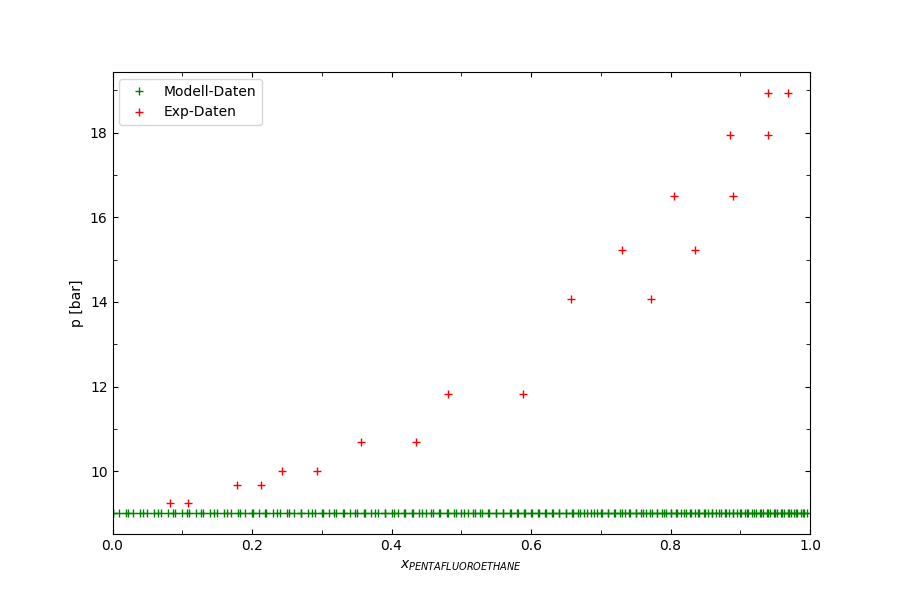
\includegraphics[scale=0.6]{PENTAFLUOROETHANE_DIMETHYL ETHER_isotherm_313.15_}
	\caption{Isothermes Phasengleichgewicht bei $ 315$.$15$ K für das Stoffgemisch Pentaflourethan|Dimethylether}
	\label{fig: phasenggw fehler2}
\end{figure}
Der Grund für das Auftreten dieses Fehlers liegt vermutlich in der \texttt{TREND} Methode, da bei sonstigen Fehlern ein Fehlercode generiert wird und die Berechnung fehlschlägt. Dieses Phänomen tritt bei einer Vielzahl an Gemischen auf, wie den im Ordner \texttt{Diagramme/<Modellname>} erzeugten Phasendiagrammen  entnommen werden kann.

Weitere mögliche Ursachen für abweichende Noten können die für das Modell verwendeten Parameter sein. Alle in dieser Arbeit verwendeten Parameter sind im Ordner \texttt{TREND 4.0} an ihrer entsprechen Stelle zu finden und liegen dem Quellcode bei.

Zusätzlich zur Behebung der auftretenden Fehler gibt es an einigen Stellen noch Verbesserungspotential. Dies betrifft hauptsächlich die Berechnung der Punkte der Phasengleichgewichte. Es ist sinnvoll die experimentellen Daten mit der \texttt{TREND} Routine \texttt{TREND\_EOS\_FIT} zu berechnen, da diese Methode Ergebnisse bei genau gleichem Druck oder genau gleicher Temperatur berechnen kann. Um diesen Ansatz verfolgen zu können, muss gewährleistet sein, dass die experimentellen Daten in der Datenbank in der korrekten Orientierung vorliegen. Konkret heißt das, dass sichergestellt werden muss, dass die angegebenen Molenbrüche sich auf die erste Komponente des Gemischs beziehen. Das ist aktuell bei einigen Gemischen nicht der Fall. Erst wenn dieser Schritt erledigt ist, kann die Routine zur Berechnung des Phasengleichgewichts angepasst und die dann nicht mehr notwendige Methode zur Bestimmung der Lage des Phasengleichgewichts entfernt werden. 


\end{document}
